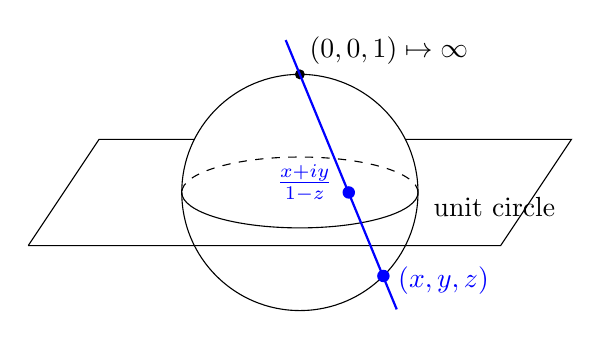
\begin{tikzpicture}[scale=1.5]
  % equatorial plane (back edge broken where the sphere is in front)
  \draw (-2.3,-0.45) -- (1.7,-0.45) -- (2.3,0.45) -- (0.893,0.45);
  \draw (-0.893,0.45) -- (-1.7,0.45) -- (-2.3,-0.45);
  % sphere and unit circle (equator)
  \draw (0,0) circle (1);
  \draw (-1,0) arc (180:360:1 and 0.3);
  \draw[dashed] (1,0) arc (0:180:1 and 0.3);
  \node[right] at (1.05,-0.12) {unit circle};
  % north pole
  \fill (0,1) circle (1.2pt);
  \node[above right] at (0,1) {$(0,0,1)\mapsto\infty$};
  % projection line through the north pole
  \draw[blue, thick] (-0.12,1.29) -- (0.82,-0.99);
  \fill[blue] (0.414,0) circle (1.5pt);
  \fill[blue] (0.707,-0.707) circle (1.5pt);
  \node[blue, right] at (0.75,-0.75) {$(x,y,z)$};
  \node[blue, left] at (0.36,0.08) {$\frac{x+iy}{1-z}$};
\end{tikzpicture}
